%!TEX root = ../thesis.tex


\begin{figure}[!b]
    \centering
    \begin{subfigure}[t]{0.9 \textwidth}
        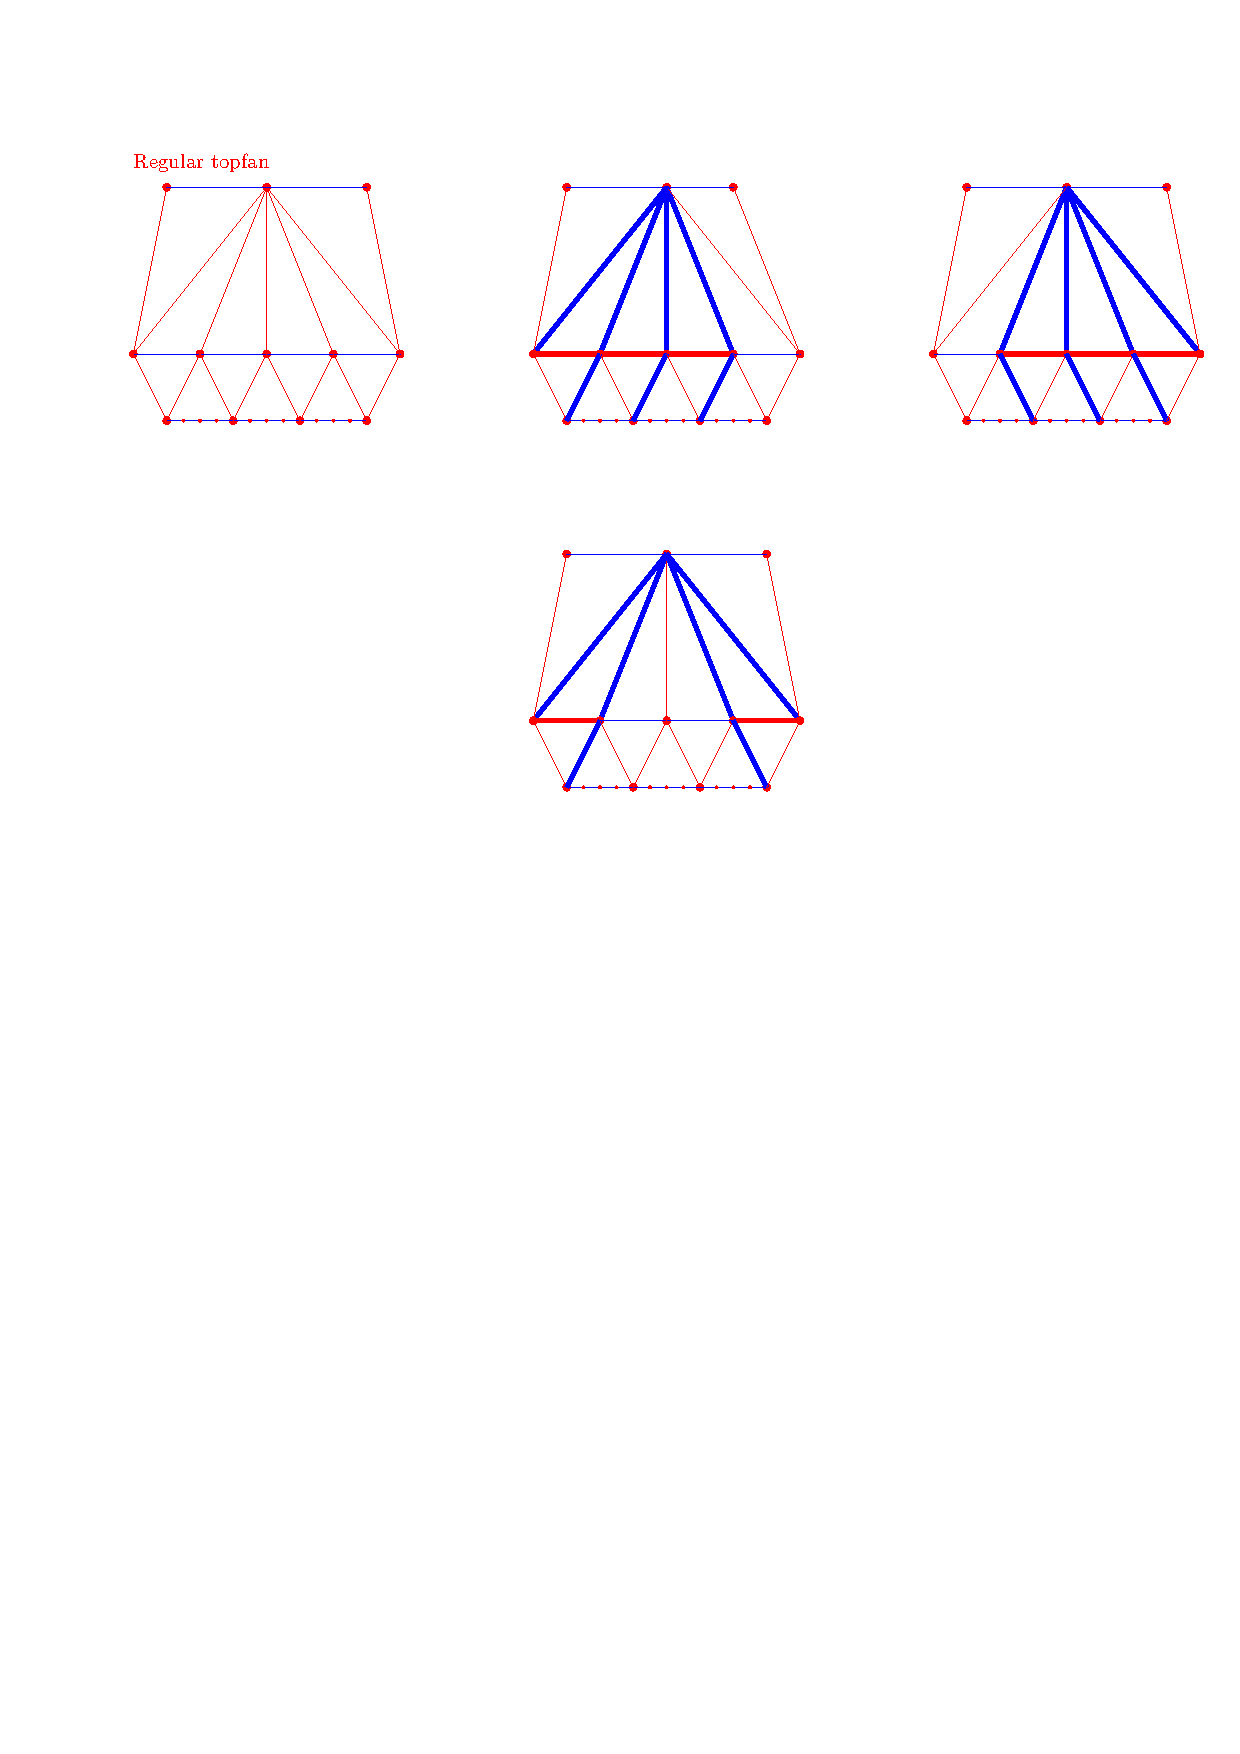
\includegraphics[width = \textwidth]{topFanFlips/img/regular}
        \caption{The regular topfan flip.}
        \label{fig:fanflip:regular}
    \end{subfigure}
    ~
    \centering
    \begin{subfigure}[t]{0.45 \textwidth}
        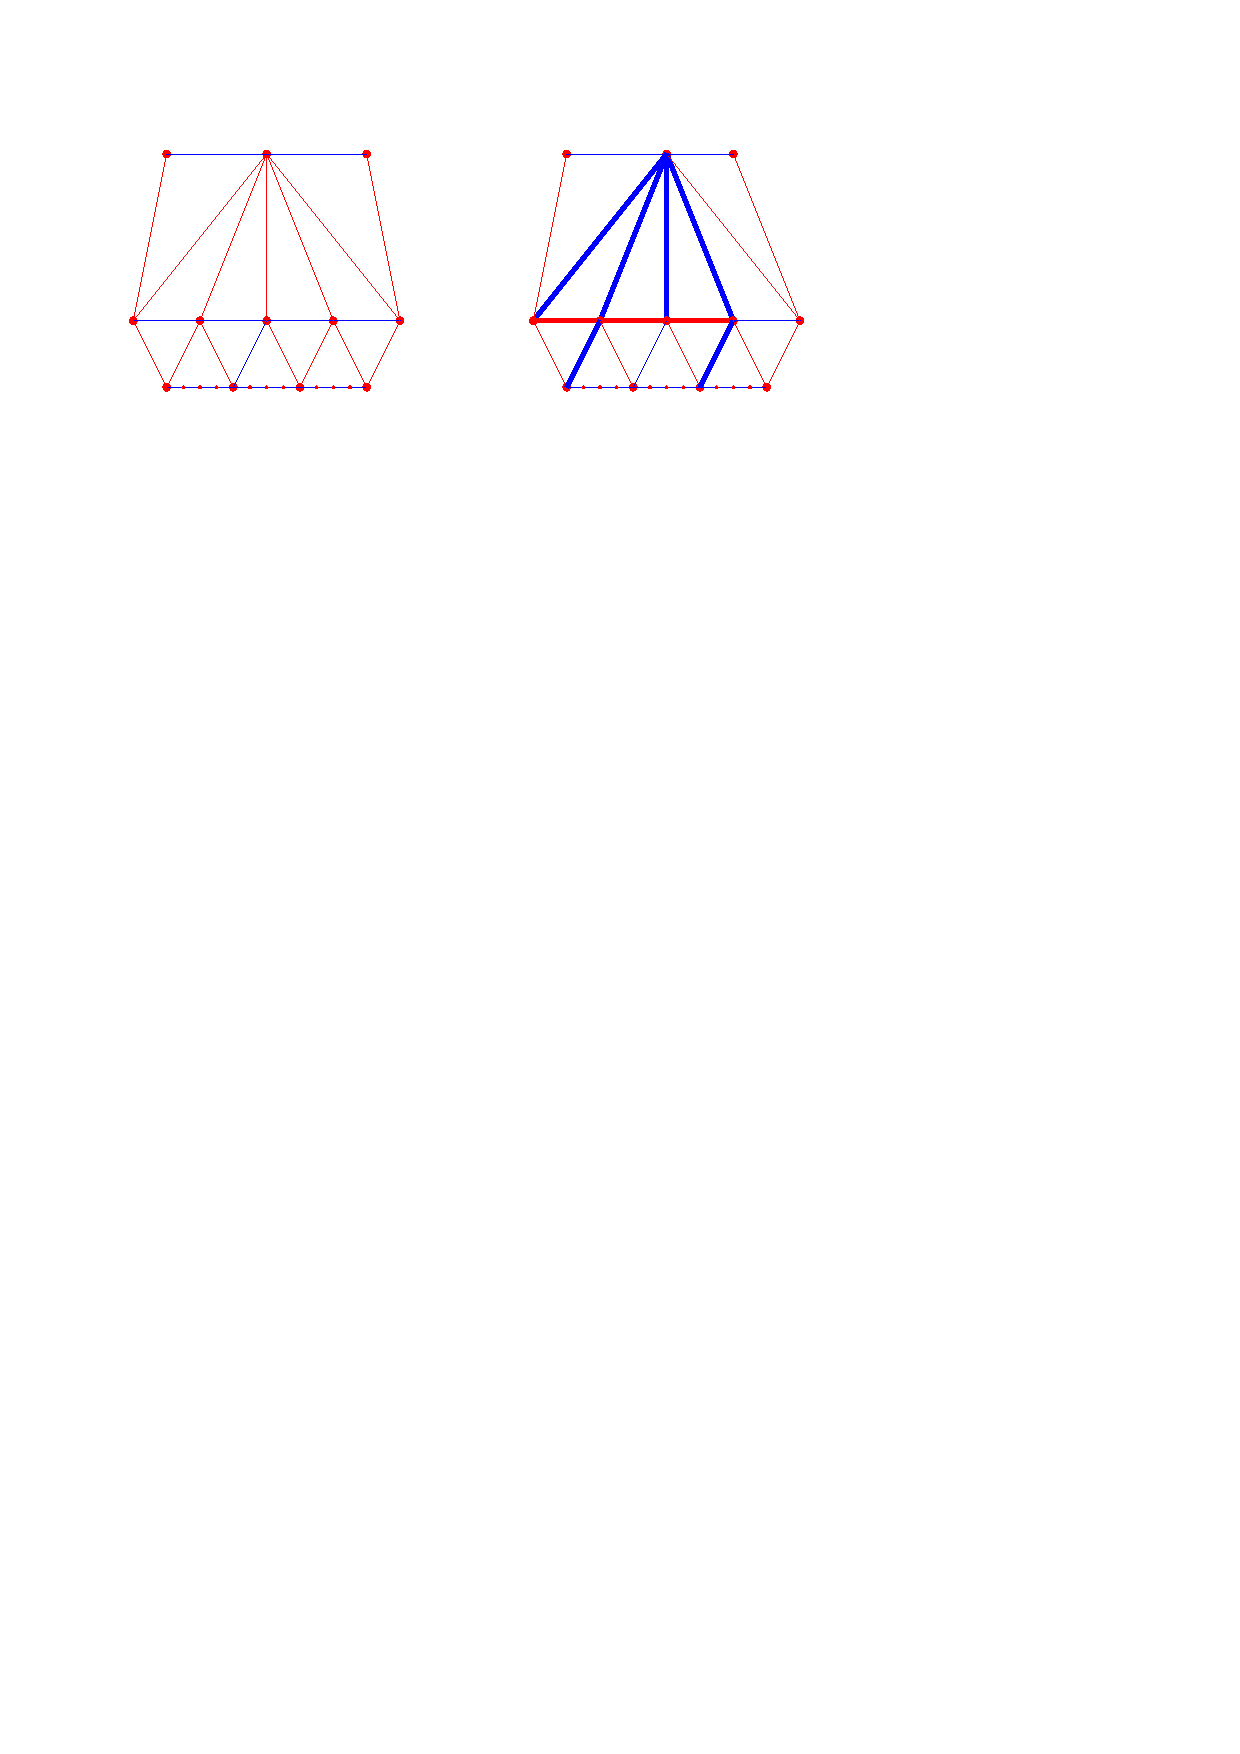
\includegraphics[width = \textwidth]{topFanFlips/img/merge}
        \caption{Topfan flip above a merge.}
        \label{fig:fanflip:merge}
    \end{subfigure}
    ~
    \begin{subfigure}[t]{0.45 \textwidth}
        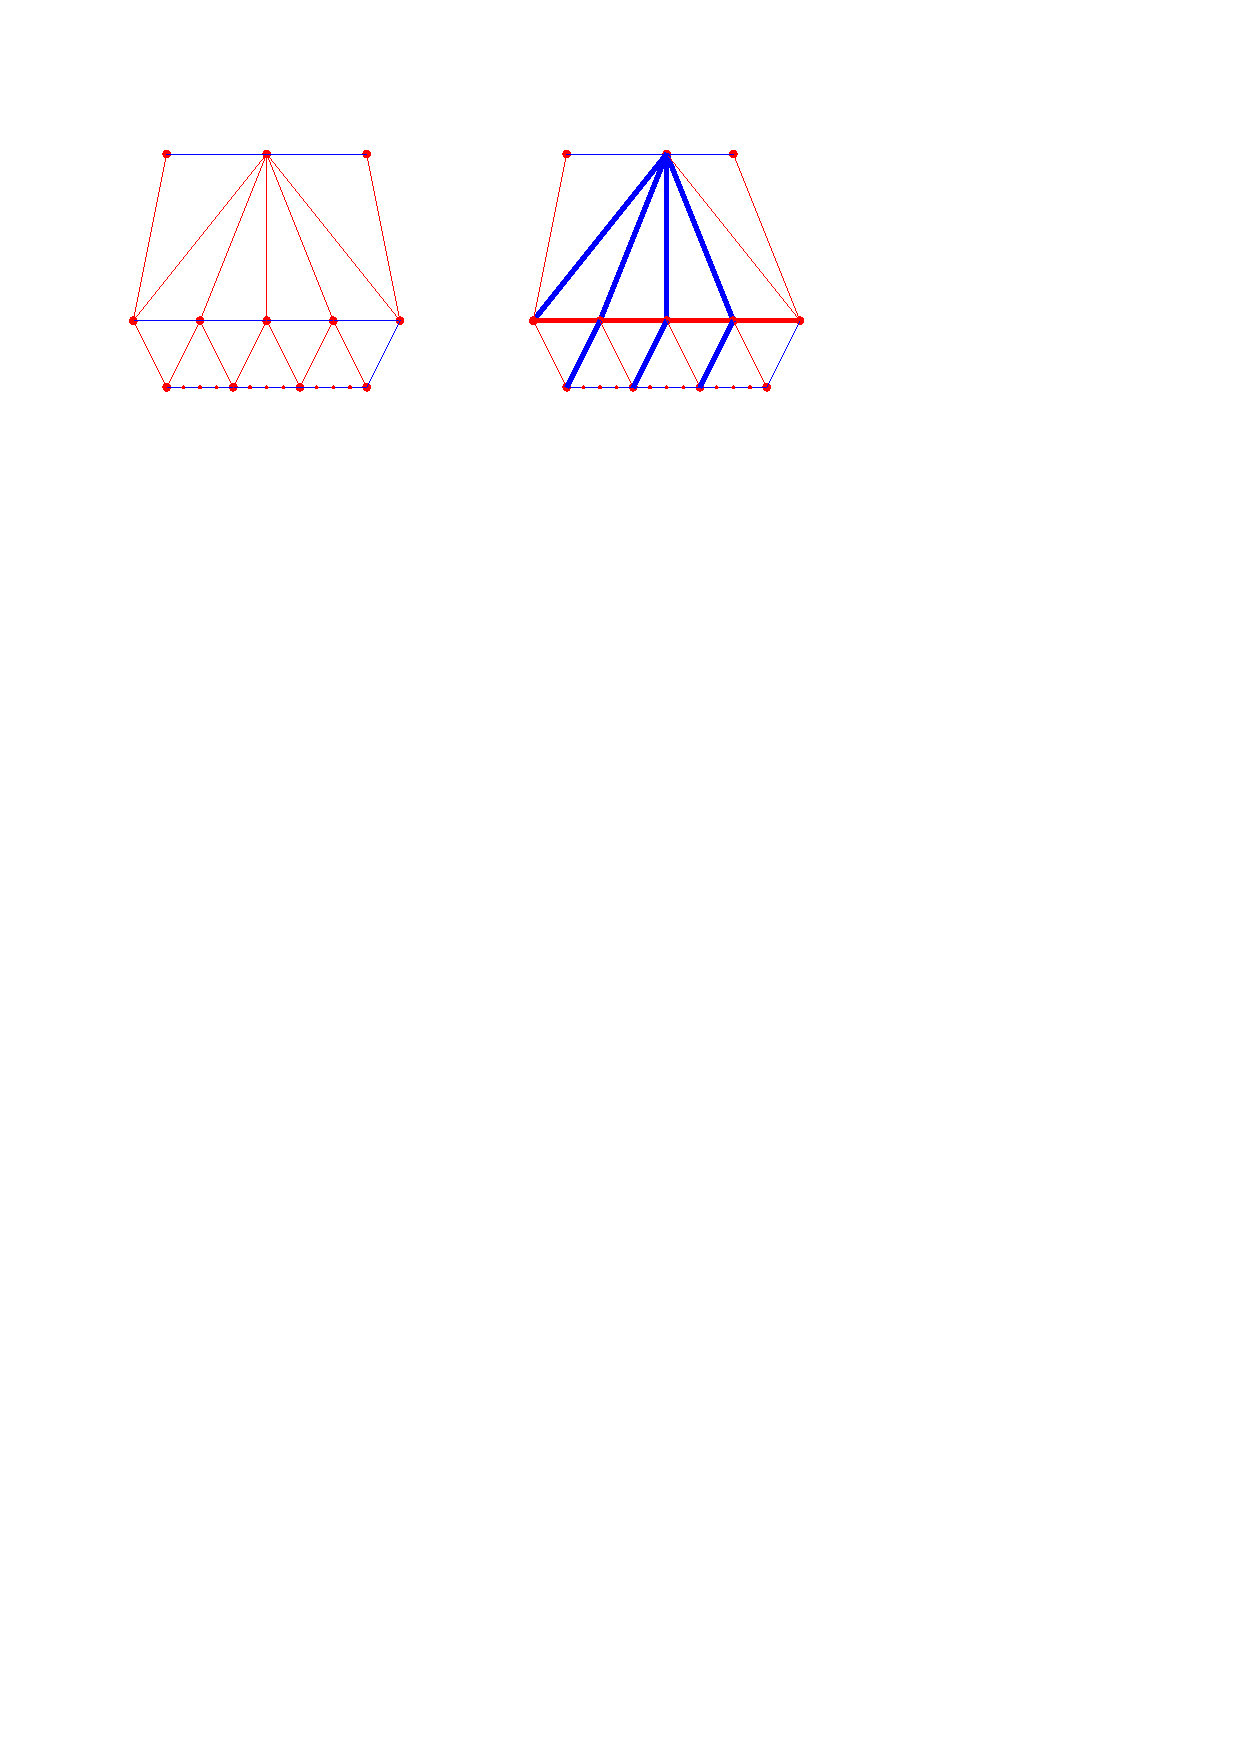
\includegraphics[width =\textwidth]{topFanFlips/img/mergeend}
        \caption{Topfan flip next to merge. Note the additional red edge.}
        \label{fig:fanflip:mergeLastVertex}
    \end{subfigure}
    \centering
    \begin{subfigure}[t]{0.45 \textwidth}
        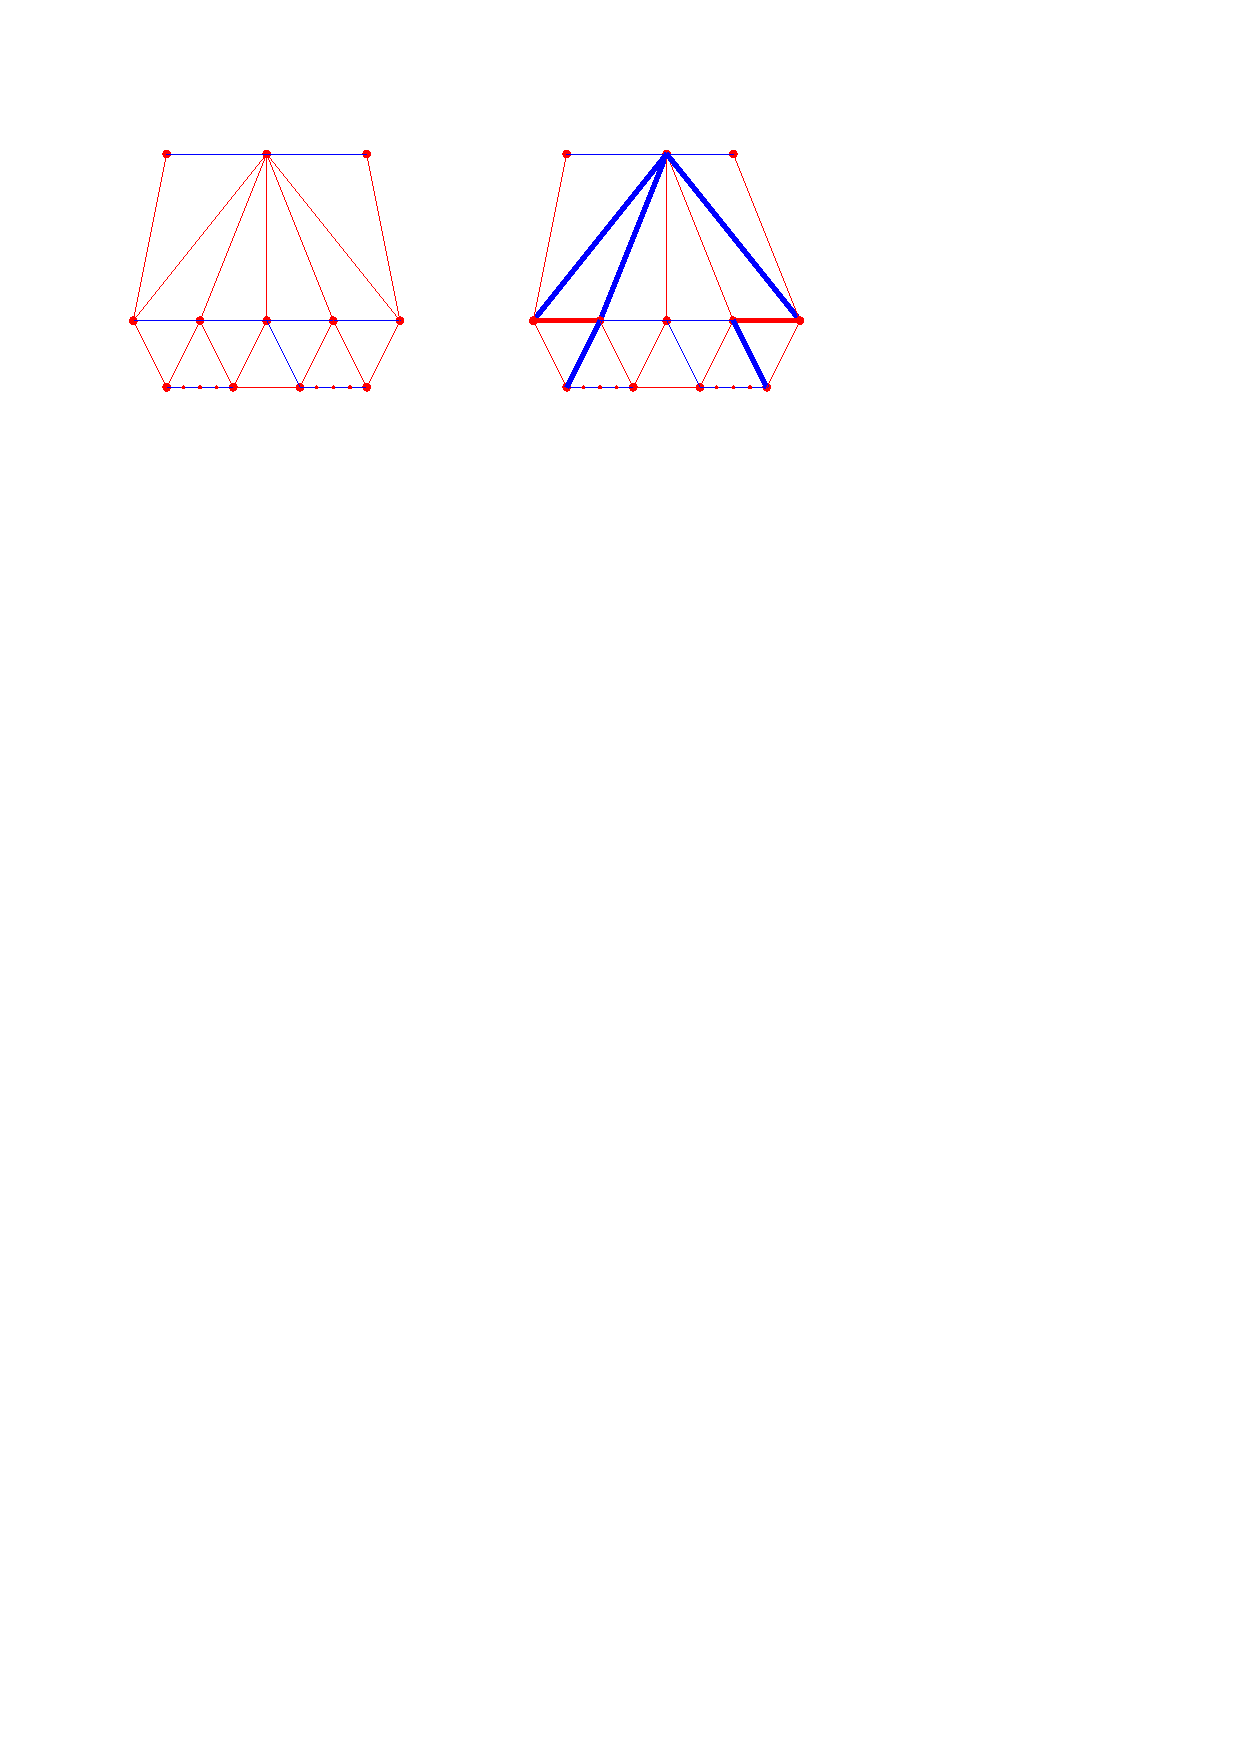
\includegraphics[width = \textwidth]{topFanFlips/img/split}
        \caption{Before a split we stop.}
        \label{fig:fanflip:split}
    \end{subfigure}
    ~
    \begin{subfigure}[t]{0.45 \textwidth}
        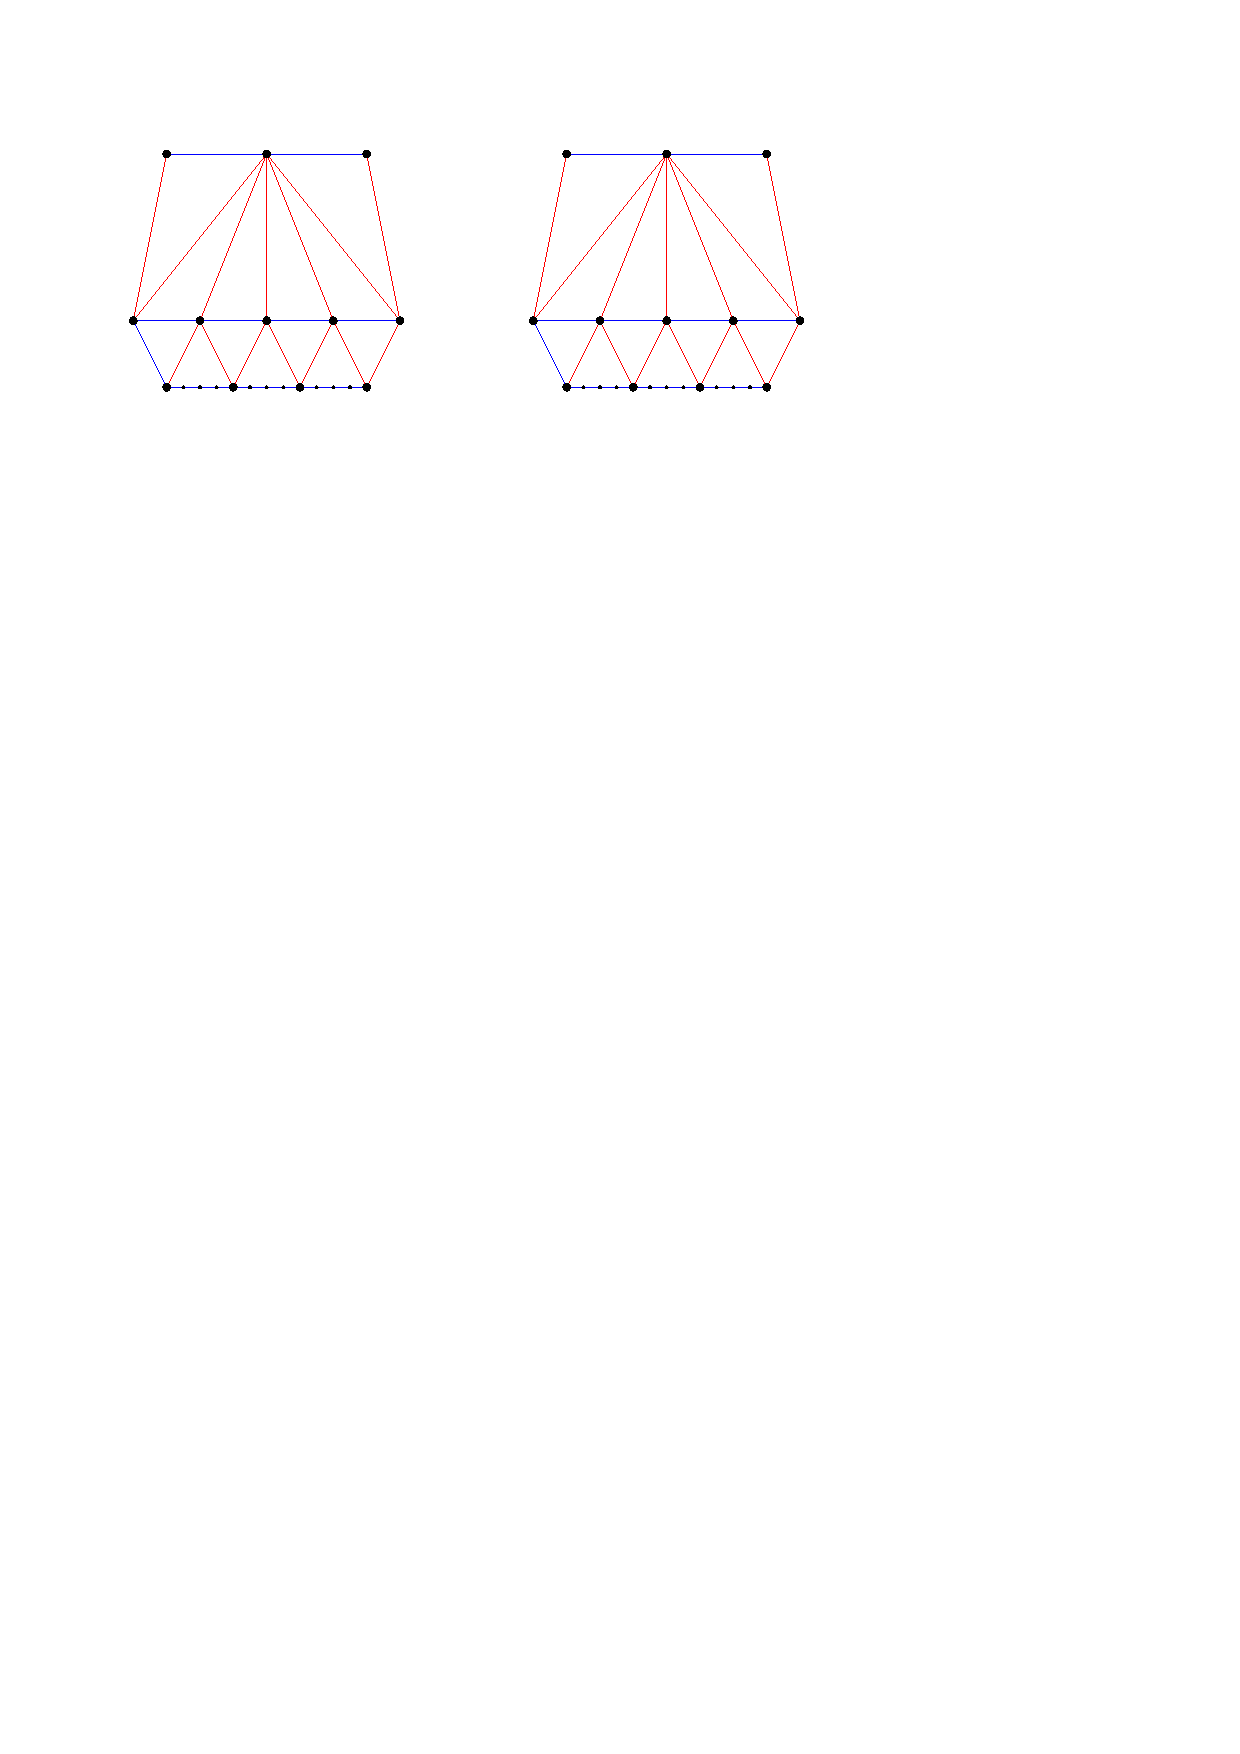
\includegraphics[width =\textwidth]{topFanFlips/img/splitfront}
        \caption{If the split is on the first vertex we do not flip at all.}
        \label{fig:fanflip:splitFirstVertex}
    \end{subfigure}

    \caption{Topfan Flips.}
    \label{fig:fanflip:fanflips}
\end{figure}

\subsection{Topfan flips}
\thispagestyle{plain}
\label{ss:fanflip}

\mypar{Overview}
In Section~\ref{ss:flipBlueZ}, we obtained a vertically one-sided regular edge labeling (Lemma \ref{lm:sweep:vertOnsided}), moreover, this regular edge labeling never has a split vertex next to a topfan handle along a bottom path (Lemma \ref{lm:zflip:NoTwoSplitsAboveEachOtherVertOnesided}).
Using local recoloring (\emph{flips}) on the topfans we will maintain a one-sided regular edge labeling (Lemma \ref{lm:topfan:oneSidedREL}) and make sure that large topfans only occur in very specific situations (Lemma \ref{lm:topfan:remainingTopfans}). It will turn out that we can deal with these specific situations in the final step of the algorithm described in Section~\ref{ss:subdiv}.
Our flips differ depending on whether we encounter a split and or merge in the bottom boundary path.
Refer to Figure~\ref{fig:fanflip:fanflips} for a first glance at the different kinds of topfan flips.


\mypar{In what order do we flip topfans}
  We would like to start at the bottommost face $F$. We can unfortunately no longer use the creation order since the removal of blue $Z$'s may have changed which faces lie above which other faces, they may even have merged faces.
  Hence, we have to show that there always is a face $F$ whose whole top boundary path borders faces that are not treated while its bottom boundary path borders no such faces.

  \begin{lemma}
    \label{lm:top:order}
    There is a face $F$ such that the whole top boundary path of $F$ borders faces that are not treated while the bottom boundary path does not border such faces.
  \end{lemma}
  \begin{proof}
    Let us first remove all treated faces from $\ext G$ by removing their blue edges and connecting their red edges with $S$.

    Unless there are no faces remaining, and in that case we are finished, there is at least one \emph{splitvertex} (vertex with at least two outgoing blue edges) and one \emph{mergevertex} (vertex with at least two blue incoming edge) along the directed path formed by the vertices adjacent to $\pS$.
    There can be no merges before the first split, nor splits after the last merge. Because there is nowhere for these blue paths to come from or go, respectively.
    Hence, somewhere along the path there is a split followed by a merge.
    This face has a bottom boundary path that is entirely adjacent to $\pS$ after removing treated faces.
    The top boundary path borders untreated faces.
  \end{proof}

  We keep considering the bottommost untreated face, until ther are no faces left. We know that this face is below only untreated face by Lemma~\ref{lm:top:order}. Since a topfan flip only affects the current face and faces below it we never have to flip in a face that is affected by the results of a topfan flip.

  We do not flip topfans whose fanhandle is adjacent to the merge of the face.

\mypar{How to flip a topfan}
  A topfan is above a number of edges of the bottom boundary path of the blue face containing the topfan. These edges are the rim of the fan. We will call a vertex \emph{$\pS$-adjacent} if it adjacent to $\pS$.

  We flip the edges of the topfan along the rim starting at the first vertex and ending at the vertex \textbf{before} the first splitvertex or $\pS$-adjacent vertex or the vertex \textbf{before} the last vertex. This can imply that we do not flip any edges (in the case that the first vertex is a split vertex or $\pS$-adjacent).

  We will use the notation introduced in figure \ref{fig:fanflip:regular}.
  For the first vertex $v_1$ we recolor the adjacent outer edge of the topfan. For subsequent vertices $v_i$ we recolor the rim edge between this vertex and the previous vertex $v_{i-1}$ red and we recolor both edges directly adjacent to this edge in the angular order of $v_i$ blue (if they were not already blue).
  If we stop flipping before a merge vertex $v_{i+1}$ we flip an additional edge $v_i v_{i+1}$ along the rim, in order to prevent a blue $Z$ from forming.

\mypar{Examples}
  Let us show a few examples of this procedure to improve clarity.
  If the rim has no merges or splits, we execute the topfan flip depicted in Figure~\ref{fig:fanflip:regular}.
  We color all but the rightmost fan edge blue, color all but the rightmost rim edge red and color the left outer edges of all topfans below this topfan in the face below the current face blue.

  If the rim consists of merges and regular vertices, we easily adept a topfan flip to this situation. We simply do not flip the edge merging in as depicted in Figure~\ref{fig:fanflip:merge}.
  A special case is given by a merge on the last vertex on the bottom edges of the topfan. In that case we flip all rim edges (even the last one) to prevent a blue $Z$ from forming. See figure \ref{fig:fanflip:mergeLastVertex}.

  Splits are more difficult to handle. We are unfortunately unable to keep flipping once we hit a split hence we stop before we get that far. See Figure~\ref{fig:fanflip:split}. It this happens on the first vertex we do not flip at all, see Figure~\ref{fig:fanflip:splitFirstVertex}.

\mypar{The result}
  Before the topfanflips, we had a vertically one-sided regular edge labeling. Afterwards we still have a vertically one-sided regular edge labeling, as we will prove in Lemma \ref{lm:topfan:oneSidedREL}. Moreover, we have no large top-fans except for some controlled cases (Lemma \ref{lm:topfan:remainingTopfans}).

  \begin{lemma}
    \label{lm:topfan:oneSidedREL}
    The regular edge labeling is still vertically one-sided after a topfan flip.
  \end{lemma}
  \begin{proof}
    We take another look at Figure~\ref{fig:fanflip:fanflips}. Note that due to Lemma \ref{lm:zflip:blueZNorVertOneSided} a regular edge labeling is vertically one-sided as long as there is no blue $Z$.  Since the graph was one-sided we can assume that we had no blue $Z$'s.
    Let us first consider the regular case. Since the edge  $v_n w_m$ is red, (otherwise we would have a merge) this change does not produce any blue $Z$'s.

    The merge case, due to the clever recoloring, also does not lead to a blue $Z$.
    It is clear the split cases do not produce a blue $Z$ either.
    Since any $\pS$-adjacent fan is treated like a split fan, we also do not create $Z$'s in these cases.
  \end{proof}
\pagebreak[2]

\begin{lemma}
  \label{lm:topfan:remainingTopfans}
  In the remaining faces every large topfan is in one of the following two situations:
  \begin{enumerate}
    \item  This topfan is at the start of the face.
    \item  The left outer rim vertex is a splitvertex.
  \end{enumerate}
\end{lemma}
\begin{proof}
  All topfans are manipulated in such a way that they start a new face, or are colored blue entirely, unless the left outer rim vertex is a split. Since in that case we do not flip at all, but then the left outer rim vertex is indeed a split.
\end{proof}
